\section{Ferro-ressonância}

Os efeitos de ferro-ressonância estão presentes em capacitores e indutores com capacidade de sofrerem saturação. Dessa forma, assim como a ressonância normal, em que ocorre a partir do circuito ser excitado com uma tensão cuja frequência seja próxima ou igual à sua frequência natural, a ferro-ressonância se dará de forma semelhante. No regime de ferro-ressonância há uma variação rápida e descontínua nas amplitudes e fases das correntes e tensões de operação, resultando em formas de onda não senoidais (pode conter harmônicas) e com altos valores de pico e sobrefluxo no núcleo do transformador podendo prejudicar os equipamentos.

Situações de ferro-ressonância são:

\begin{itemize}
    \item Ressonância entre cabos de elevada capacitância e reatores limitadores de corrente;
    \item Ressonância entre indutância linear e a capacitância de um sistema com linha levemente carregada;
    \item Ferro-ressonância entre TP's e a capacitância entre os enrolamentos de um transformador de distribuição;
    \item Ferro-ressonância em sistemas com elementos saturáveis e filtros harmônicos.
\end{itemize}

Para ilustrar a ferro-ressonância, imagina-se um circuito RLC série alimentado por uma fonte senoidal. Normalmente para um valor fixo de indutância, só haverá um ponto de ressonância para o circuito. Porém, se introduzir uma indutância variável de acordo com a saturação, haverá uma faixa de valores em que ocorrerá ressonância. A figura \ref{slide5:rlc} ilustra ambos os casos, para (a) o caso da indutância fixa e (b) para o caso da indutância variável, marcando o ponto de maior corrente.

\begin{figure}[H]
\begin{center}
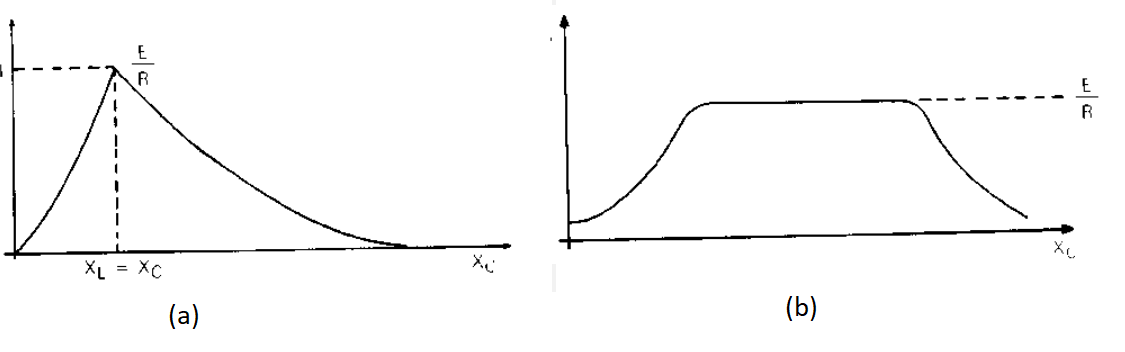
\includegraphics[width=12cm]{images/RLC.png}
\caption{Circuito RLC para (a) indutância fixa e (b) indutância variável.}
\label{slide5:rlc} 
\end{center}
\end{figure}

Outra forma de ilustrar é a partir de um circuito LC. Pela lei de Kirchhoff de tensões, tem-se:

\begin{center}
    $E = V_C + V_L$
\end{center}

A tensão na fonte $E$, a tensão no capacitor $V_C = -I X_C$ negativa, pois tem sinal trocado em relação às quedas de tensão nos indutores da rede, com circuito circulado pela corrente $I$ e tensão no indutor de $V_L$. O equivalente de Thévenin enxergando apenas o indutor é: $E_t = E+IX_C$. Esse valor é importante para se traçar uma curva linear da solução ideal do circuito e compará-la com o caso da curva de saturação dada em \ref{slide5:sat}.

\begin{figure}[H]
\begin{center}
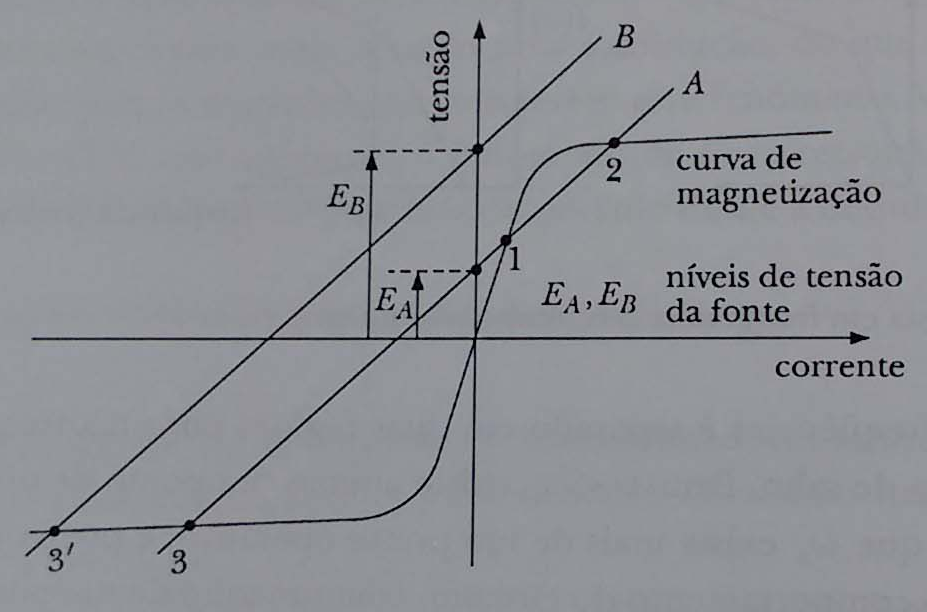
\includegraphics[width=8cm]{images/sat.png}
\caption{Circuito LC pelo equivalente de Thévenin, com comportamento linear e não-linear sobreposto..}
\label{slide5:sat} 
\end{center}
\end{figure}

Analisando a figura acima, o caso A possui três soluções e o B apenas uma, com apenas a solução 1 da curva A apresentando equilíbrio para variações pequenas de corrente, enquanto que para as demais, uma menor variação de corrente resultará em uma operação durante a saturação, resultando em sobretensão.

Demais casos de circuitos que podem sofrer ferro-ressonância são:

\begin{itemize}
    \item Gerador alimentando circuitos com acoplamento capacitivo, porém com presença de TP;
    \item Gerador alimentando linha de transmissão alimentando TP, em que chave seccionadora aberta na linha causa acoplamento capacitivo;
    \item Gerador alimentando linha com transformador trifásico ligado em $Y-Y$, $\Delta-Y$ aterrado, etc.
\end{itemize}

Algumas soluções para o caso de ferro-ressonância são:

\begin{itemize}
    \item Trocar chaves fusíveis por disjuntores, evitando desbalanceamento de fases no sistema;
    \item Manobrar, por último, quando possível, o transformador mais próximo, evitando o circuito série de cabo-transformador;
    \item Alocar cargas resistivas no secundário do transformador, de forma que quando refletida no primário irá aumentar o amortecimento do circuito, porém danosamente aumentando o carregamento do cabo e do transformador ao aumentar a dissipação de potência;
    \item Modificação do circuito por aumentar o comprimento do cabo, alimentação aérea, reator de terciário, ou aumentando a resistência do aterramento, porém resulta em investimentos elevados;
    \item Ou reduzir a tensão aplicada para evitar que o transformador opere na saturação.
\end{itemize}